\documentclass[10pt,a4paper]{book}

\NewDocumentCommand\Yc{}{\mathbb{Y}}
\NewDocumentCommand\Zc{}{\mathbb{Z}}
\NewDocumentCommand\fava{}{\texttt{fava}}
\DeclareMathOperator*{\app}{\enspace\xrightarrow[\beta]{}\enspace}
\lstdefinelanguage{sample}{keywords={fava,true,false,compile,sudo,pacman,git,java},otherkeywords={=>},string=[b]{"},morecomment=[l]//}

\book{Scalaで自作するプログラミング言語処理系}{Computation Models {\&} Compilers on Scala}{2}{自作言語,パーサコンビネータ,構文解析,PEG}

\begin{document}
\maketitle
\tableofcontents

\chapter{言語処理系を作る}

本書では、\textbf{ラムダ計算}を理論的背景に持つ独自のプログラミング言語の\textbf{インタプリタ}を自作して、\textbf{計算論}の基礎を学ぶ。
実装は公開済みで気軽に閲覧できる。最低限の機能に留めた簡素な言語だが、改良次第では汎用的な言語に拡張できる。

\begin{Verbatim}{bash}
$ git clone https://github.com/nextzlog/fava
\end{Verbatim}

改良には開発環境が必要だが、殆どの場合は\textbf{パッケージリポジトリ}経由で、即座に調達できる。ArchLinuxの例を示す。

\begin{Verbatim}{bash}
$ sudo pacman -S jdk-openjdk scala
\end{Verbatim}

頒布版には、\textbf{対話環境}を同梱した。また、\chapref{automata}に述べる様々な計算モデルの実験機能も同梱した。起動時に機能を選ぶ。

\begin{Verbatim}{sample}
$ java -jar build/libs/fava.jar
which language do you use?
[0]: fava
[1]: math
select: 0
fava$ "HELLO, WORLD!"
HELLO, WORLD!
\end{Verbatim}

自作言語の名前は\fava{}とする。専用の命令を実装した仮想的な実行環境で動作する。算術演算や論理演算が実行できる。

\begin{Verbatim}{sample}
fava$ 11 + 4 * 5 - 14
17
\end{Verbatim}

理念的には\textbf{純粋関数型言語}に分類できる。式に\textbf{副作用}がなく、式の値は定数で、式の構造から明確に求まる特徴を持つ。
また、関数は関数の引数や返り値にできる。ただし、関数は名前も局所変数も定義できず、数学的な関数の概念に似る。

\begin{Verbatim}{sample}
fava$ ((x)=>(y)=>3*x+7*y)(2)(3)
27
\end{Verbatim}

実用的な計算が困難な程の制約に思えるが、実際には\chapref{lambda}で解説する通り、優れた計算能力を持つ。階乗も計算できる。

\begin{Verbatim}{sample}
fava$ ((f)=>((x)=>f(x(x)))((x)=>f(x(x))))((f)=>(n)=>(n==0)?1:n*f(n-1))(10)
3628800
\end{Verbatim}

理論的には、\textbf{帰納的に枚挙可能}な集合に対する、任意の計算を実行できる。自然数を関数で表現する芸当も可能である。

\begin{Verbatim}{sample}
fava$ ((f,x)=>f(f(f(f(f(x))))))((x)=>x+1,0) // 0 + 1 + 1 + 1 + 1 + 1
5
\end{Verbatim}

また、任意の\textbf{順序組}を定義して操作できる。順序組は構造体と等価である。理論的には複雑な\textbf{グラフ構造}も表現できる。

\begin{Verbatim}{sample}
fava$ ((pair)=>pair((car,cdr)=>car))(((car,cdr)=>(z)=>z(car,cdr))(12,34))
12
fava$ ((pair)=>pair((car,cdr)=>cdr))(((car,cdr)=>(z)=>z(car,cdr))(12,34))
34
\end{Verbatim}

対話環境の拡張機能として、実行環境で実行される命令列を表示する機能も用意した。実行環境の動作の理解に役立つ。

\begin{Verbatim}{sample}
fava$ compile(1 + 2)
Push(1) Push(2) Add
\end{Verbatim}

\chapter{計算モデルを作る\label{chap:automata}}

\textbf{言語処理系}とは、言語仕様に沿って書かれた計算手順を読み取り、任意の計算機を構築または模倣する\textbf{万能機械}である。
計算機を抽象化した数学的な模型を\textbf{計算モデル}と呼ぶ。例えば、論理回路は\sectref{regex}に述べる\textbf{有限状態機械}で表現できる。

\section{有限状態機械\label{sect:regex}}

有限状態機械は、\textbf{状態}と\textbf{遷移規則}の有限集合で構成される。論理回路で言えば、\textbf{記憶素子}が保持する情報が状態である。
有限状態機械に信号$x_n$を与えると、\tabref{state}の遷移規則に従って、状態$q_n$から状態$q_{n+1}$に遷移して、信号$y_n$を返す。

\begin{table}[h]
\centering
\caption{state transition tables.\label{tab:state}}
\subfloat[SR flip-flop.\label{tab:state:SR}]{
\begin{tabular}{CCCC} \toprule
$x_n$ & $q_n$ & $q_{n+1}$ & $y_n$ \\ \midrule
00 & 0 & 0 & 0 \\
00 & 1 & 1 & 1 \\
01 & 0 & 0 & 0 \\
01 & 1 & 0 & 1 \\
10 & 0 & 1 & 0 \\
10 & 1 & 1 & 1 \\
11 & 0 & - & - \\
11 & 1 & - & - \\ \bottomrule
\end{tabular}
}
\subfloat[JK flip-flop.\label{tab:state:JK}]{
\begin{tabular}{CCCC} \toprule
$x_n$ & $q_n$ & $q_{n+1}$ & $y_n$ \\ \midrule
00 & 0 & 0 & 0 \\
00 & 1 & 1 & 1 \\
01 & 0 & 0 & 0 \\
01 & 1 & 0 & 1 \\
10 & 0 & 1 & 0 \\
10 & 1 & 1 & 1 \\
11 & 0 & 1 & 0 \\
11 & 1 & 0 & 1 \\ \bottomrule
\end{tabular}
}
\subfloat[2bit counter.\label{tab:state:2c}]{
\begin{tabular}{CCCC} \toprule
$x_n$ & $q_n$ & $q_{n+1}$ & $y_n$ \\ \midrule
0 & 00 & 00 & 00 \\
1 & 00 & 01 & 00 \\
0 & 01 & 01 & 01 \\
1 & 01 & 10 & 01 \\
0 & 10 & 10 & 10 \\
1 & 10 & 11 & 10 \\
0 & 11 & 11 & 11 \\
1 & 11 & 00 & 11 \\ \bottomrule
\end{tabular}
}
\end{table}

有限状態機械が受け取る信号列を\textbf{文}と見做す場合もある。これを言語処理に応用する体系が、\chapref{math}の\textbf{言語理論}である。
有限状態機械には、それに対応する\textbf{正規表現}が必ず存在する。この性質を利用して、正規表現の処理系を実装してみる。

\begin{Verbatim}{Scala}
class R[S](val test: Seq[S] => Option[Seq[S]])
\end{Verbatim}

正規表現は、正規表現を結合して、帰納的に定義できる。その最小単位が以下に示す\texttt{One}型で、特定の1文字に適合する。

\begin{Verbatim}{Scala}
case class One[S](r: S) extends R[S](Some(_).filter(_.head == r).map(_.tail))
\end{Verbatim}

適合すると、残りの文字列を返す。ここに別の正規表現を適用すれば、正規表現の連結を意味する。これが\texttt{Cat}型である。
\texttt{Alt}型は、正規表現の選択肢を表す。これは、遷移先の状態が複数ある状況を表す。これを遷移規則の\textbf{非決定性}と呼ぶ。

\begin{Verbatim}{Scala}
case class Cat[S](l: R[S], r: R[S]) extends R[S](seq => l.test(seq).map(r.test).flatten)
case class Alt[S](l: R[S], r: R[S]) extends R[S](seq => l.test(seq).orElse(r.test(seq)))
\end{Verbatim}

\texttt{Opt}型は、指定された正規表現の省略可能な出現を表す。また、\texttt{Rep}型は、指定された正規表現の0回以上の反復を表す。

\begin{Verbatim}{Scala}
case class Opt[S](r: R[S]) extends R[S](seq => r.test(seq).orElse(Some(seq)))
case class Rep[S](r: R[S]) extends R[S](seq => Cat(r, Opt(Rep(r))).test(seq))
\end{Verbatim}

正規表現\texttt{Z(L+|G)O}に相当する、有限状態機械の実装例を示す。\sectref{regex}の内容を応用すれば、言語処理系も実装できる。

\begin{Verbatim}{Scala}
val ZLO = Cat(One('Z'), Cat(Alt(Rep(One('L')), One('G')), One('O')))
println(if(ZLO.test("ZLLLLLLLLLLLLLLLLO").isDefined) "OK" else "NO")
\end{Verbatim}

\section{セルオートマトン\label{sect:cell}}

単体の有限状態機械は、再帰計算が苦手である。しかし、その集合体である\textbf{セルオートマトン}は、任意の計算ができる。
構成単位を\textbf{セル}と呼ぶ。各セルは、近傍$k$個のセルの状態を参照し、\eqref{cell}に示す遷移規則$\delta$に従って、状態遷移する。
%
\begin{equation}
\label{eq:cell}
\delta: Q^k \to Q.
\end{equation}
%
空間的な自由を得た恩恵で、再帰構造を持つ計算に対応する。例えば、\textbf{フラクタル図形}を描画する遷移規則が存在する。
\figref{langton}に示す\textbf{ラングトンの環}の例では、仮足を伸ばして\eqref{loop}の遺伝子を注入し、分裂増殖する生物群集を模倣する。
%
\begin{equation}
\label{eq:loop}
0710710711111041041071071071.
\end{equation}

\begin{figure}[h]
\centering
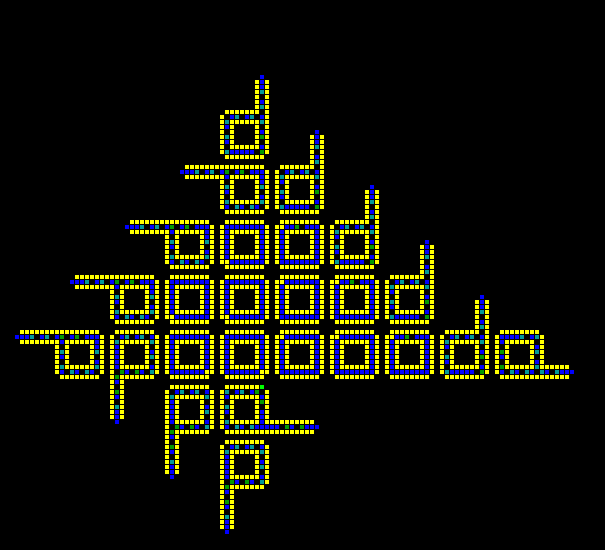
\includegraphics[width=\linewidth]{images/cell.loops.eps}
\caption{Langton's loops in cellular automata.\label{fig:langton}}
\end{figure}

2次元の実装例を示す。遷移規則は引数で指定する。全てのセルが同時に更新される\textbf{同期型セルオートマトン}を採用した。

\begin{Verbatim}{Scala}
class CA2[S](rule: Seq[Seq[S]] => S, d: Int = 1) {
	def ROI[V](i: Int)(s: Seq[V]) = Range.inclusive(i - d, i + d).map(Math.floorMod(_, s.size)).map(s)
	def apply(s: Seq[Seq[S]]) = s.indices.map(x => s(x).indices.map(y => rule(ROI(x)(s).map(ROI(y)))))
}
\end{Verbatim}

理論的には、任意の遷移規則を初期状態で受け取り、模倣する万能機械も構築できる。その例が\textbf{ワイヤワールド}である。
黒の基板に黄色の配線を作ると、信号が配線を巡り、記憶素子を含む、様々な論理回路を模倣する。\figref{wire}に例を示す。

\begin{figure}[h]
\centering
\subfloat[4bit counter.\label{fig:wire:count}]{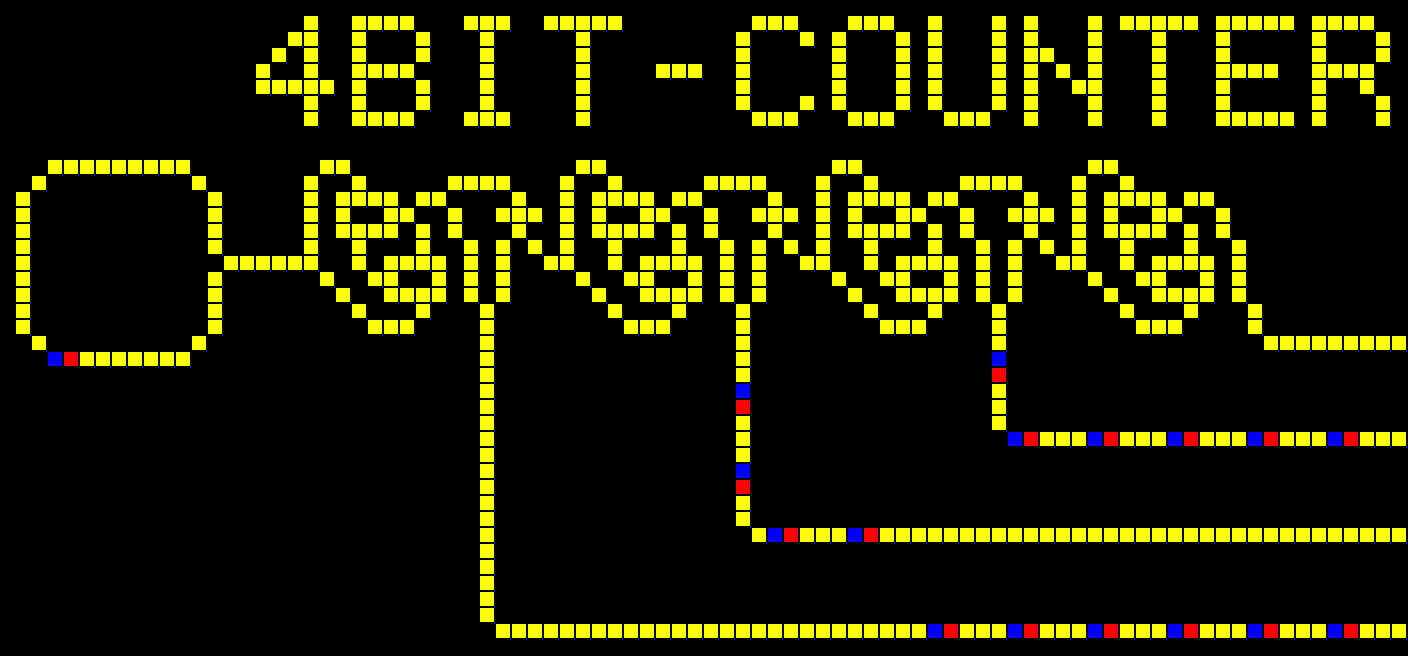
\includegraphics[width=\linewidth]{images/wire.count.eps}}\\
\subfloat[binary adder.\label{fig:wire:adder}]{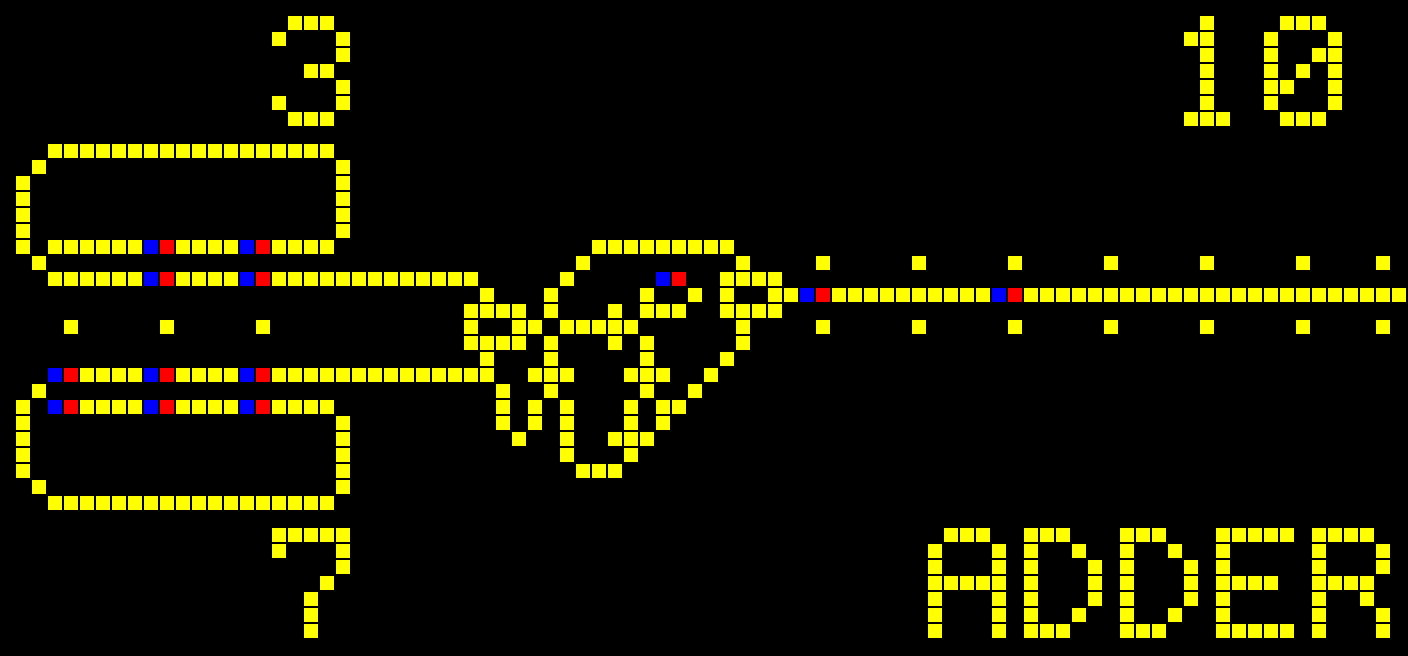
\includegraphics[width=\linewidth]{images/wire.adder.eps}}
\caption{Wireworld logic circuits.\label{fig:wire}}
\end{figure}

\subfigref{wire}{count}は\textbf{カウンタ}である。左側の\textbf{発振回路}から周期的に信号を送り込む度に、右側の配線4本の信号が切り替わる。
\subfigref{wire}{adder}は\textbf{加算器}である。果ては、表示器を備えた計算機さえ実装可能な点が特徴だが、遷移規則は実に単純である。

\begin{Verbatim}{Scala}
object WireWorldRule extends CA2[Char](ROI => ROI(1)(1) match {
	case 'W' if(ROI.flatten.count(_ == 'H') == 1) => 'H'
	case 'W' if(ROI.flatten.count(_ == 'H') == 2) => 'H'
	case 'W' => 'W'
	case 'H' => 'T'
	case 'T' => 'W'
	case 'B' => 'B'
})
\end{Verbatim}

\section{チューリング機械\label{sect:turing}}

\textbf{チューリング機械}は、無限長の\textbf{テープ}と、その内容を読み書きする有限状態機械と、\eqref{tape}の遷移関数$\delta$で構成される。
状態$q_n$で記号$x_n$を読み取ると、記号$y_n$に書き換える。状態$q_{n+1}$に遷移して$\lambda_n$の方向に移動し、再び記号を読み取る。
%
\begin{equation}
\label{eq:tape}
(q_{n+1},y_n,\lambda_n) = \delta(q_n,x_n),
\where
\left\{
\begin{aligned}
q_n &\in Q,\\
x_n,y_n &\in \Sigma,\\
\lambda_n &\in \{L,R\}.
\end{aligned}
\right.
\end{equation}
%
この動作は、任意の逐次処理型の計算機と等価であり、並列処理型のセルオートマトンと並んで、計算機の頂点に立つ。
特に、帰納的に枚挙可能な集合の計算が得意である。2進数で与えられた自然数の後続を求める手順を、\figref{tape}に示す。

\begin{figure}[h]
\centering
\subfloat[\texttt{100=011+001}.]{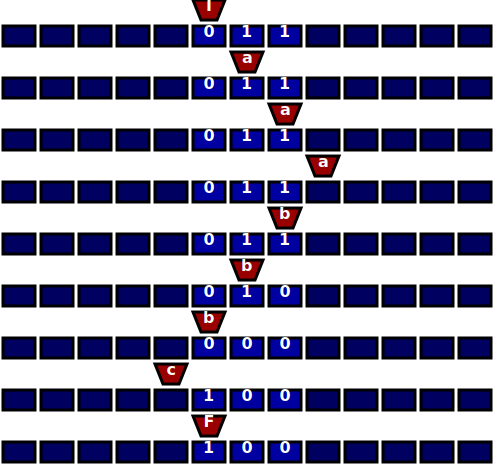
\includegraphics[width=.5\linewidth]{images/tape.plus1.eps}}
\subfloat[\texttt{110=101+001}.]{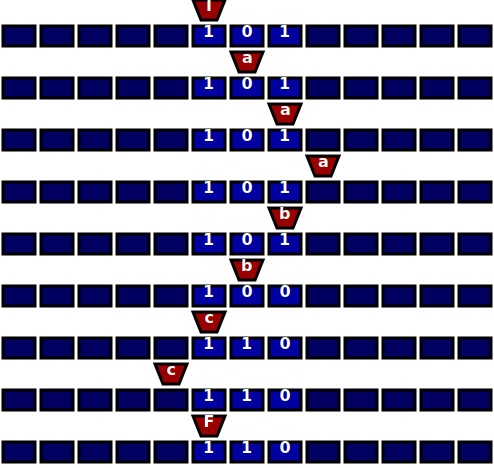
\includegraphics[width=.5\linewidth]{images/tape.plus2.eps}}
\caption{numerical increment operation on a Turing machine ($k=1$).\label{fig:tape}}
\end{figure}

任意の遷移関数を読み取り、その遷移関数を忠実に実行する、言語処理系と等価な\textbf{万能チューリング機械}も実装できる。
遷移関数と計算手順で、別々のテープを使用した例を\texttt{UTM}型に実装する。状態F0からF1にかけ、遷移規則を検索する。

\begin{Verbatim}{Scala}
class UTM[V](data1: Seq[V], data2: Seq[V], bk1: V, bk2: V, mvL: V, mvR: V, var st1: V) {
	val tape1 = data1.zipWithIndex.map(_.swap).to(collection.mutable.SortedMap)
	val tape2 = data2.zipWithIndex.map(_.swap).to(collection.mutable.SortedMap)
	var (hd1, hd2) -> st2 = (0, 0) -> "F0"
	def rd1 = tape1.getOrElse(hd1, bk1)
	def rd2 = tape2.getOrElse(hd2, bk2)
	def apply(stop: V) = Iterator.continually(st2 match {
		case "F0" if rd2 == st1 => (st1 = st1, st2 = "F1", tape1(hd1) = rd1, hd1 += 0, hd2 += 1)
		case "F0" if rd2 != st1 => (st1 = st1, st2 = "F0", tape1(hd1) = rd1, hd1 += 0, hd2 += 5)
		case "F1" if rd2 == rd1 => (st1 = st1, st2 = "F2", tape1(hd1) = rd1, hd1 += 0, hd2 += 1)
		case "F1" if rd2 != rd1 => (st1 = st1, st2 = "F0", tape1(hd1) = rd1, hd1 += 0, hd2 += 4)
		case "F2" if rd2 != bk2 => (st1 = rd2, st2 = "F3", tape1(hd1) = rd1, hd1 += 0, hd2 += 1)
		case "F3" if rd2 != bk2 => (st1 = st1, st2 = "F4", tape1(hd1) = rd2, hd1 += 0, hd2 += 1)
		case "F4" if rd2 == bk1 => (st1 = st1, st2 = "F5", tape1(hd1) = rd1, hd1 += 0, hd2 += 1)
		case "F4" if rd2 == mvL => (st1 = st1, st2 = "F5", tape1(hd1) = rd1, hd1 -= 1, hd2 += 1)
		case "F4" if rd2 == mvR => (st1 = st1, st2 = "F5", tape1(hd1) = rd1, hd1 += 1, hd2 += 1)
		case "F5" if rd2 == bk2 => (st1 = st1, st2 = "F0", tape1(hd1) = rd1, hd1 += 0, hd2 += 1)
		case "F5" if rd2 != bk2 => (st1 = st1, st2 = "F5", tape1(hd1) = rd1, hd1 += 0, hd2 -= 1)
	}).takeWhile(t => st1 != stop || st2 != "F0").map(t => tape1.values.mkString)
}
\end{Verbatim}

状態F2からF4で、状態遷移と書き戻しと移動を行う。状態F5でテープの左端に戻り、状態F0に戻る。使用例を示す。

\begin{Verbatim}{Scala}
case class CUTM(data1: String, data2: String) extends UTM(data1, data2, ' ', '*', 'L', 'R', 'I')
CUTM("0111111", "I0a0RI1a1Ra0a0Ra1a1Ra b Lb0c1Lb1b0Lb F1 c0c0Lc1c1Lc F R")('F').foreach(println)
\end{Verbatim}

遷移規則は\eqref{tape}の通り、5個組で読み込ませる。初期状態\texttt{I}から状態\texttt{F}まで動かすと、\figref{tape}の計算が実行される。

\section{逆ポーランド記法\label{sect:pola}}

\textbf{スタック}を備え、再帰計算に対応した有限状態機械を\textbf{プッシュダウンオートマトン}と呼ぶ。\eqref{push}の遷移関数$\delta$に従う。
$Q$は状態の、$\Sigma$と$\Gamma$は入力とスタックの記号の有限集合である。$\Gamma^*$は$\Gamma$の元を並べた任意長の記号列$y^*$の集合である。
%
\begin{equation}
\label{eq:push}
(q_{n+1},y^*_n) = \delta(q_n,\sigma_n,x_n),
\where
\left\{
\begin{aligned}
q_n &\in Q,\\
x_n &\in \Gamma,\\
y^*_n &\in \Gamma^*,\\
\sigma_n &\in \Sigma.
\end{aligned}
\right.
\end{equation}
%
記号$\sigma_n$を受け取ると、スタックの先頭の記号$x_n$を取り除き、先頭に記号列$y^*_n$を順番に積んで。状態$q_{n+1}$に遷移する。
再帰計算を活用した例として、\sectref{regex}で実装した正規表現の拡張を考える。以下の関数\texttt{ZLO}は、記号列$\texttt{Z}^n\texttt{L}\texttt{O}^n$を表す。

\begin{Verbatim}{Scala}
def ZLO: R[Char] = Cat(One('Z'), Cat(Alt(One('L'), new R(ZLO.test(_))), One('O')))
println(ZLO.test("ZZZZZZZZZZZZZZZZZZZZZZZZZLOOOOOOOOOOOOOOOOOOOOOOOOO").isDefined)
\end{Verbatim}

残念ながら、再帰計算は実行できても、受け取った記号列を読み返す機能がなく、計算能力はチューリング機械に劣る。
ただし、記憶装置としてスタックを使う広義の\textbf{スタック機械}は、重要な計算モデルである。\eqref{math}の計算を例に考える。
%
\begin{equation}
\label{eq:math}
(1 + 2) * (10 - 20).
\end{equation}
%
演算子には優先順位があるため、式を左から読むだけでは、計算は困難である。数値を保持する記憶装置も必要である。
前者は、\eqref{pola}の\textbf{逆ポーランド記法}で解決する。演算子に優先順位はなく、出現する順番に、直前の数値に適用される。
%
\begin{equation}
\label{eq:pola}
\texttt{1 2 + 10 20 - *}.
\end{equation}
%
手順を\figref{math}に示す。逆ポーランド記法は、式の読み返しを伴う再帰計算や条件分岐を除き、任意の計算を実行できる。

\begin{figure}[h]
\centering
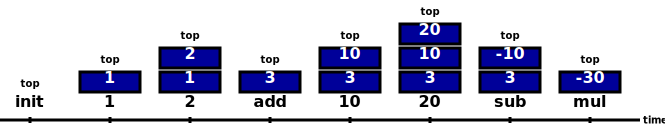
\includegraphics[width=\linewidth]{images/pola.anime.eps}
\caption{\texttt{1 2 + 10 20 - *}.\label{fig:math}}
\end{figure}

その再帰計算や条件分岐も、指定された長さだけ記号列を遡る\textbf{分岐命令}があれば実現できる。詳細は\chapref{call}に解説する。
逆ポーランド記法の数式を計算する実装例を示す。数式は、空白で区切る必要がある。この実装は、\chapref{math}で再び使う。

\begin{Verbatim}{Scala}
object ArithStackMachine extends collection.mutable.Stack[Int]() {
	def apply(program: String): Int = program.split(" +").map {
		case "+" => push(((a: Int, b: Int) => b + a)(pop, pop))
		case "-" => push(((a: Int, b: Int) => b - a)(pop, pop))
		case "*" => push(((a: Int, b: Int) => b * a)(pop, pop))
		case "/" => push(((a: Int, b: Int) => b / a)(pop, pop))
		case num => this.push(num.toInt)
	}.lastOption.map(_ => pop).last
}
\end{Verbatim}

\chapter{ラムダ計算の理論\label{chap:lambda}}

実在する計算機を意識した\chapref{automata}の計算モデルに対し、関数の\textbf{評価}と\textbf{適用}による計算手順の抽象化がラムダ計算である。
\chapref{lambda}では、任意の式を\textbf{ラムダ式}と呼ぶ。変数も、整数も、関数もラムダ式である。関数は、\eqref{abs}のように定義する。
%
\begin{equation}
\label{eq:abs}
f \coloneqq \lambda xy.2x+3y+z+1.
\end{equation}
%
\eqref{abs}を関数$f$の\textbf{ラムダ抽象}と呼ぶ。変数$x$と$y$を、$\lambda$により\textbf{束縛}された変数と呼ぶ。また、変数$z$を\textbf{自由変数}と呼ぶ。
\eqref{abs}は\eqref{curry}と等価である。関数$g$は、変数$x$を束縛し、変数$y$を引数に取る関数を返す。これを\textbf{カリー化}と呼ぶ。
%
\begin{equation}
\label{eq:curry}
g \coloneqq \lambda x.\lambda y.2x+3y+1.
\end{equation}
%
\eqref{app}は、変数$x$と$y$を具体的な値で束縛する。これを関数適用と呼ぶ。また、式の実体を計算する操作を評価と呼ぶ。
評価の途中で、束縛変数を定数に置換する操作を\textbf{ベータ簡約}と呼ぶ。\eqref{app}の値は、2度の簡約を経由して$27$と求まる。
%
\begin{equation}
\label{eq:app}
\lambda x.\lambda y.(3x+7y) \enspace 2 \enspace 3 \app \lambda y.(6+7y) \enspace 3 \app 6+21 = 27.
\end{equation}
%
任意の自然数と演算は、自然数を枚挙する関数$s$と自然数$0$があれば、\textbf{ペアノの公理}で定義できる。\eqref{num}に例を示す。
自然数は、2個の引数を取る関数で表す。変数$x$に自然数を渡せば、加算になる。変数$s$に自然数を渡せば、乗算になる。
%
\begin{equation}
\label{eq:num}
n \coloneqq \lambda sx.(s^{\circ n}x) \enspace \lambda x.(x+1) \enspace 0,
\enspace
\left\{
\begin{aligned}
a + b &\coloneqq \lambda ab.\lambda sx.as(bsx),\\
a \times b &\coloneqq \lambda ab.\lambda sx.a(bs)x.
\end{aligned}
\right.
\end{equation}
%
真偽値は、真と偽の順序組を引数に取り、どちらかを返す関数で表現できる。論理積と論理和の定義例を\eqref{bool}に示す。
真偽値の変数$y$を偽で束縛すれば、変数$x$との論理積になる。逆に、変数$x$を真で束縛すれば、変数$y$との論理和になる。
%
\begin{equation}
\label{eq:bool}
\mathrm{t} \coloneqq \lambda xy.x, \enspace
\mathrm{f} \coloneqq \lambda xy.y, \enspace
\left\{
\begin{aligned}
a \land b &\coloneqq \lambda ab.ab\mathrm{f},\\
a \lor  b &\coloneqq \lambda ab.a\mathrm{t}b.
\end{aligned}
\right.
\end{equation}
%
関数$f$に対し、性質$f(x)\!=\!x$を満たす点$x$を\textbf{不動点}と呼ぶ。また、\eqref{fix}の性質を満たす関数$p$を\textbf{不動点演算子}と呼ぶ。
%
\begin{equation}
\label{eq:fix}
\forall f, \enspace f(p(f)) \equiv p(f).
\end{equation}
%
関数$p$を利用すれば、再帰的な関数$h(x)$を\eqref{rec}で定義できる。関数$h$は、再帰計算の実体を表す関数$g$を引数に取る。
%
\begin{equation}
\label{eq:rec}
h \coloneqq \lambda x.pgx, \where g \coloneqq \lambda fy.E.
\end{equation}
%
関数$h$が再帰的であるには、関数$g$の変数$f$が関数$h$を参照する必要がある。\eqref{fixed}の変形で、この要求は保証される。
%
\begin{equation}
\label{eq:fixed}
h
\equiv \lambda x.(pg) x
\equiv \lambda x.(g (pg)) x
\equiv \lambda x.ghx.
\end{equation}
%
\eqref{fixed}を\textbf{無名再帰}と呼ぶ。関数$p$が実装できれば、任意の再帰計算を実行できる。最も著名な実装例を\eqref{Y}に示す。
%
\begin{equation}
\label{eq:Y}
\Yc{} \coloneqq \lambda f.(\lambda x.f(xx))(\lambda x.f(xx)).
\end{equation}
%
関数$f$に対し、\eqref{Y}の関数$\Yc$が\eqref{fix}を満たす様子は、\eqref{Yf}で証明できる。ただし、無限再帰に注意を要する。
関数$\Yc{}f$を評価すると、同じ関数$\Yc{}f$が右辺に出現する。無限再帰を防ぐには、関数$\Yc{}f$の評価を遅延させる必要がある。
%
\begin{equation}
\label{eq:Yf}
\Yc{}f
\app (\lambda x.f(xx))(\lambda x.f(xx))
\app f((\lambda x.f(xx))(\lambda x.f(xx)))
\equiv f(\Yc{}f).
\end{equation}
%
または、\eqref{Z}の関数$\Zc$なら、関数$\Zc{}f$の評価は停止する。関数$\Zc{}$は、関数$\Yc$に\textbf{イータ変換}の逆を施した関数である。
%
\begin{equation}
\label{eq:Z}
\mathrm{Z} \coloneqq \lambda f.(\lambda x.f(\lambda y.xxy))(\lambda x.f(\lambda y.xxy)).
\end{equation}
%
関数$\Zc{}f$を評価すると、変数$y$を引数に取る関数が出現する。右辺の関数$\Zc{}f$の展開が保留され、無限再帰は回避される。
%
\begin{equation}
\label{eq:Zf}
\mathrm{Z}f
\app (\lambda x.f(\lambda y.xxy))(\lambda x.f(\lambda y.xxy))
\app f(\lambda y.(\lambda x.f(\lambda y.xxy))(\lambda x.f(\lambda y.xxy))y)
\app f(\lambda y.\mathrm{Z}fy).
\end{equation}
%
\eqref{Y}の関数$\Zc$を利用すれば、本書で自作する言語は、任意の計算を実行できる。\chapref{favac}で実装を終えた後に実験する。

\chapter{簡単なコンパイラ\label{chap:math}}

\chapref{automata}の計算モデルは、C言語やラムダ計算など\textbf{高水準言語}の内容を実行するには原始的すぎる。そこで、翻訳を行う。
翻訳を行う言語処理系を\textbf{コンパイラ}と呼ぶ。\chapref{math}では、簡単な逆ポーランド記法の翻訳を例に、その概念を解説する。

\section{形式言語の階層性\label{sect:lang}}

\textbf{形式言語}とは、定義が明確で、何らかの計算手順で処理できる言語である。まず、形式言語$L$は\eqref{lang}で定義される。
%
\begin{equation}
\label{eq:lang}
L(G) \subset \Sigma^* = \left\{\langle\sigma_1,...,\sigma_n,...\rangle\mid\sigma_n\in\Sigma\right\}.
\end{equation}
%
言語$L$は\textbf{文}の集合である。文とは、記号$\sigma$の列である。記号は有限集合$\Sigma$で定義され、集合$\Sigma$を\textbf{アルファベット}と呼ぶ。
記号$\sigma$の出現には、明確な規則がある。この規則を\textbf{生成規則}と呼び、生成規則の集合を\textbf{文法}と呼ぶ。\eqref{gen}に例を示す。
%
\begin{equation}
\label{eq:gen}
P = \left\{
\begin{aligned}
\mathtt{S} &\to \texttt{(S)},\\
\mathtt{S} &\to \texttt{(f)},
\end{aligned}
\right.:(N\cup\Sigma)^*\to(N\cup\Sigma)^*.
\end{equation}
%
生成規則は、左辺の記号列を右辺の記号列に置換する規則である。\eqref{gen}の例では、記号\texttt{S}から\eqref{fs}が導出される。
%
\begin{equation}
\label{eq:fs}
\texttt{(f)},
\texttt{((f))},
\texttt{(((f)))},
\texttt{((((f))))},
\texttt{(((((f)))))},
\texttt{((((((f))))))},
\texttt{(((((((f)))))))},
\texttt{((((((((f))))))))},
\ldots.
\end{equation}
%
生成規則の両辺に出現できる記号$\nu\!\in\!N$を\textbf{非終端記号}と呼ぶ。また、右辺に限って出現する記号$\sigma\!\in\!\Sigma$を\textbf{終端記号}と呼ぶ。
任意の文は、\textbf{開始記号}と呼ばれる記号$S$を起点に生成される。最終的に、言語$L(G)$の文法$G$は\eqref{gram}で定義される。
%
\begin{equation}
\label{eq:gram}
G=(N,\Sigma,P,S),\where S\in N.
\end{equation}
%
文法$G$に従う文を生成し、または文を開始記号$S$に帰する手順が定義され、曖昧性がなければ、文法$G$は\textbf{形式的}である。
形式言語の中でも、生成規則が自由な言語を\textbf{帰納的可算言語}と呼び、\eqref{csg}の制限を加えた言語を\textbf{文脈依存言語}と呼ぶ。
%
\begin{equation}
\label{eq:csg}
\alpha A \beta \to \alpha \gamma \beta,
\where
\left\{
\begin{aligned}
A &\in N,\\
\alpha,\beta &\in (N\cup\Sigma)^*,\\
\gamma &\in (N\cup\Sigma)^+.
\end{aligned}
\right.
\end{equation}
%
形式言語の中でも、\eqref{cfg}の制限を持ち、前後の文脈に依存せずに、生成規則が適用できる言語を\textbf{文脈自由言語}と呼ぶ。
\sectref{pola}で述べたプッシュダウンオートマトンを利用して、文に対して生成規則を再帰的に適用することで処理できる。
%
\begin{equation}
\label{eq:cfg}
A \to \alpha,
\where
\left\{
\begin{aligned}
A &\in N,\\
\alpha &\in (N\cup\Sigma)^*.
\end{aligned}
\right.
\end{equation}
%
形式言語の中でも、文法の制約が強く、有限状態機械で処理可能な言語を\textbf{正規言語}と呼ぶ。その記法が正規表現である。
有限状態機械では、無限の記憶を持てず、特に再帰的な生成規則を扱えず、生成規則は\eqref{reg}に示す形式に制限される。
%
\begin{equation}
\label{eq:reg}
\left\{
\begin{aligned}
A &\to a,\\
A &\to aB,
\end{aligned}
\right.
\where
\left\{
\begin{aligned}
a &\in \Sigma,\\
A,B &\in N.
\end{aligned}
\right.
\end{equation}
%
形式言語の文は、適用した生成規則の木構造で表現できる。これを\textbf{構文木}と呼び、構文木を導く作業を\textbf{構文解析}と呼ぶ。
特にLL法では、終端記号の列を読み進め、見つけた終端記号に適う生成規則を、開始記号$S$を起点に深さ優先探索する。
%
\begin{equation}
(S=\texttt{add})\to(\texttt{mul + mul})\to(\texttt{num * num + num})\to(\texttt{1 * 2 + 3}).
\end{equation}
%
LR法では、終端記号の列を読み進め、置換可能な部分を非終端記号に置換する。最終的に開始記号$S$に到達して終わる。
%
\begin{equation}
(\texttt{1 * 2 + 3})\to(\texttt{num * num + num})\to(\texttt{mul + mul})\to(S=\texttt{add}).
\end{equation}
%
通常、高水準言語は形式言語である。仮に自然言語を採用すると、翻訳する手順が曖昧になり、実装困難なためである。

\section{解析表現文法の例\label{sect:PEG}}

形式文法は、構文解析の際には曖昧になる。そこで、生成規則ではなく、構文解析の手順を形式的に定義した文法もある。
\textbf{解析表現文法}はその例である。解析表現文法は、文脈依存言語の部分集合を扱う。簡単な四則演算を定義する例を示す。

\begin{table}[h!]
\raggedright
\begin{tabular}{@{}Bll}
加減算 & \verb#add ::= mul (('+' / '-') mul)*# \\
乗除算 & \verb#mul ::= num (('*' / '/') num)*# \\
整数値 & \verb#num ::= [0-9]+ / '(' add ')'#
\end{tabular}
\end{table}

左辺が非終端記号で、右辺が非終端記号と終端記号の列を表す。ただし、右辺に出現する記号には、以下の意味がある。

\begin{table}[h!]
\raggedright
\begin{tabular}{@{}ll}
\verb# *# & 直前の記号が0回以上出現する。\\
\verb# +# & 直前の記号が1回以上出現する。\\
\verb# ?# & 直前の記号が出現する場合がある。\\
\verb# /# & 直前または直後の記号が出現する。\\
\verb#()# & 括弧内の記号列をひと纏めにする。\\
\verb#''# & 引用内の字句がそのまま出現する。\\
\verb#[]# & 範囲内の記号が選択的に出現する。\\
\verb# &# & 直後の記号が出現すれば成功する。\\
\verb# !# & 直後の記号が出現すれば失敗する。\\
\end{tabular}
\end{table}

解析表現文法はLL法の亜種である\textbf{再帰下降構文解析}を定義する記法である。これは、再帰的な関数で構文解析器を表す。
様々な言語を定義可能だが、非終端記号を置換すると再び左に出現する\textbf{左再帰}の言語では、無限再帰に陥る欠点がある。

\begin{table}[h]
\raggedright
\begin{tabular}{@{}Bl}
左再帰 & \verb#add ::= add ('+' / '-') mul / mul#
\end{tabular}
\end{table}

左再帰は、\textbf{左結合}の式を表す際に重要である。\eqref{left}に例を示す。左結合の式では、式の左側の演算子が優先される。
%
\begin{equation}
\label{eq:left}
1 - 2 - 3 - 4 - 5 = (((1 - 2) - 3) - 4) - 5 = -13.
\end{equation}
%
右結合にすれば無限再帰を回避できるが、式の意味が変化してしまう。反復を表す特殊記号\texttt{*}など、代替手段で回避する。

\section{構文解析器の実装\label{sect:parsec}}

\sectref{parsec}では、\sectref{regex}で解説した正規表現の処理系を改良して、解析表現文法に基づく\textbf{パーサコンビネータ}を実装する。
以下の\texttt{PEG}型を継承した\textbf{高階関数}を組み合わせ、再帰下降構文解析器を構築する。構文解析に成功すると、結果を返す。

\begin{Verbatim}{Scala}
class PEG[+M](f: String => Option[Out[M]]) {
	def skip = Reg("""\s*""".r) ~> this <~ Reg("""\s*""".r)
	def / [R >: M](q: => PEG[R]): PEG[R] = new Alt(this, q)
	def ~ [R](q: => PEG[R]): PEG[(M, R)] = new Cat(this, q)
	def <~[R](q: => PEG[R]) = this ~ q ^ (_._1)
	def ~>[R](q: => PEG[R]) = this ~ q ^ (_._2)
	def ^ [T](f: M => T) = new Map(this, f)
	def * = new Rep(this)
	def ? = new Opt(this)
	def apply(in: String) = f(in)
}
\end{Verbatim}

構文解析器は、その構文解析器で構築した構文木と、構文解析器が読み残した終端記号の列を返す。\texttt{Out}型に実装する。

\begin{Verbatim}{Scala}
case class Out[+M](m: M, in: String) {
	def tuple[R](o: Out[R]) = Out(m -> o.m, o.in)
	def apply[R](p: PEG[R]) = p(in).map(tuple(_))
	def toSome = Out(Some(m), in)
}
\end{Verbatim}

最初に、最も単純な構文解析器を実装する。\texttt{Str}型は、指定された終端記号列を左端に発見すると、その記号列を返す。
\texttt{Reg}型は、正規表現で指定された終端記号列を左端に発見すると、その記号列を返す。両者を総称して\textbf{字句解析器}と呼ぶ。

\begin{Verbatim}{Scala}
case class Str(p: String) extends PEG(s => Option.when(s.startsWith(p))(Out(p, s.substring(p.length))))
case class Reg(p: Regex) extends PEG(p.findPrefixMatchOf(_).map(m => Out(m.matched, m.after.toString)))
\end{Verbatim}

\texttt{Alt}型は、1個目の構文解析器が構文解析に成功すると、その結果を返し、失敗した場合は、2個目の構文解析器を試す。
\texttt{Cat}型は、1個目の構文解析器を試してから、読み残した終端記号列に2個目の構文解析器を試し、結果を結合して返す。

\begin{Verbatim}{Scala}
class Alt[L, R >: L](p: => PEG[L], q: => PEG[R]) extends PEG[R](s => p(s) orElse q(s))
class Cat[+L, +R](p: => PEG[L], q: => PEG[R]) extends PEG(p(_).map(_ apply q).flatten)
\end{Verbatim}

\texttt{Map}型は、指定された構文解析器を試し、その結果に対して、関数を適用する。構文木に何らかの加工を施す際に使う。
\texttt{Opt}型は、省略可能な構文を表す。指定された構文解析器を試すが、構文解析に失敗した場合でも、成功したと見做す。

\begin{Verbatim}{Scala}
class Map[+S, +T](p: => PEG[S], f: S => T) extends PEG[T](p(_).map(t => Out(f(t.m), t.in)))
class Opt[+T](p: => PEG[T]) extends PEG(s => p(s).map(_.toSome).orElse(Some(Out(None, s))))
\end{Verbatim}

\texttt{And}型と\texttt{Not}型は、先読みを行う。指定された構文解析器を試すが、読み取り位置を進めず、構文解析の成否のみを返す。
LL法でも先読み可能だが、正規表現で切り出した字句の先読みに限定されるため、解析表現文法よりも表現能力が劣る。

\begin{Verbatim}{Scala}
class And[+T](p: => PEG[T]) extends PEG(s => if(p(s).isDefined) Some(Out(None, s)) else None)
class Not[+T](p: => PEG[T]) extends PEG(s => if(p(s).isDefined) None else Some(Out(None, s)))
\end{Verbatim}

\texttt{Rep}型は、記号の反復を表す。読み取り位置を進めては構文解析を実行し、構文解析に失敗すると、結果を結合して返す。

\begin{Verbatim}{Scala}
class Rep[+T](p: => PEG[T]) extends PEG(s => {
	def ca(a: Out[T]): Out[Seq[T]] = Out(a.m +: re(a.in).m, re(a.in).in)
	def re(s: String): Out[Seq[T]] = p(s).map(ca).getOrElse(Out(Nil, s))
	Some(re(s))
})
\end{Verbatim}

次に、特殊な構文解析器を実装する。\texttt{Fold}型は、左結合する中置記法の式を表す。無限再帰を回避する代替手段である。
1個目の構文解析器は、被演算子を表す。2個目の構文解析器は演算子を表し、演算子の左右に並ぶ被演算子を結合する。

\begin{Verbatim}{Scala}
class Fold[T](p: => PEG[T], q: => PEG[(T, T) => T]) extends PEG({
	(p ~ (q ~ p).*)^(x => x._2.foldLeft(x._1)((l, r) => r._1(l, r._2)))
} apply(_))
\end{Verbatim}

最後に実装する\texttt{Sep}型は、\texttt{Rep}型の特殊な場合で、区切り文字で区切られた記号の反復を表す。区切り文字は廃棄される。

\begin{Verbatim}{Scala}
class Sep[T](p: => PEG[T], q: => PEG[_]) extends Fold[Seq[T]](p^(Seq(_)), q^(_ => _ ++ _))
\end{Verbatim}

最終的な構文解析器を、以下の\texttt{PEGs}型を継承して実装すると、文字列や正規表現は、暗黙的に構文解析器に変換される。

\begin{Verbatim}{Scala}
class PEGs {
	implicit def implicitText(p: String): PEG[String] = new Str(p).skip
	implicit def implicitRegex(p: Regex): PEG[String] = new Reg(p).skip
}
\end{Verbatim}

使用例を示す。この実装は、数式を読み取る機能に加え、逆ポーランド記法の命令列を生成する\textbf{コード生成器}も兼ねる。

\begin{Verbatim}{Scala}
object ArithPEGs extends PEGs {
	def add: PEG[String] = new Fold(mul, ("+" / "-").^(op => (a, b) => s"$a $b $op"))
	def mul: PEG[String] = new Fold(num, ("*" / "/").^(op => (a, b) => s"$a $b $op"))
	def num: PEG[String] = "[0-9]+".r / ("(" ~> add <~ ")")
	def apply(e: String) = +ArithStackMachine(add(e).get.m)
}
\end{Verbatim}

\chapter{自作言語の仕様書\label{chap:fava}}

本書で設計する\fava{}は\textbf{動的型付け}を行う言語である。データ型は、整数型と実数型と論理型と文字列型と関数型がある。
整数型は符号付き32~bit整数で、実数型はIEEE~754~(64~bit~2進数)浮動小数点数で、文字列はUTF-16で表現される。

\begin{table}[h]
\raggedright
\begin{tabular}{@{}Bl}
整数型 & \verb#int  ::= [0-9]+# \\
実数型 & \verb#real ::= [0-9]* ([0-9] '.' / '.' [0-9]) [0-9]*# \\
論理型 & \verb#bool ::= 'true' / 'false'# \\
文字列 & \verb#text ::= '"' [^"]* '"'# \\
関数型 & \verb#func ::= '(' (id (',' id)*)? ')' '=>' expr#
\end{tabular}
\end{table}

識別子は、その識別子が記述された箇所を包含し、識別子と同じ名前の引数を持つ、最も内側の関数の引数を参照する。
関数の内外で変数を宣言または代入する機能はなく、従って、識別子が参照する実体は何らかの関数の引数に限られる。

\begin{table}[h]
\raggedright
\begin{tabular}{@{}Bl}
識別子 & \verb#id ::= [@A-Z_a-z] [@0-9A-Z_a-z]*#
\end{tabular}
\end{table}

引数の値は変更不可能なため、識別子を含む式が参照する実体は、状態によらず自明である。これを\textbf{参照透明性}と呼ぶ。
複数の文を逐次的に実行する\textbf{ブロック構文}はなく、関数宣言の構文も省略した。以下に解析表現文法による定義を示す。

\begin{table}[h]
\raggedright
\begin{tabular}{@{}Bl}
ラムダ式 & \verb#expr ::= cond / or# \\
条件分岐 & \verb#cond ::= or  '?' expr ':' expr# \\
論理積   & \verb#or   ::= or  '|' and / and# \\
論理和   & \verb#and  ::= and '&' eql / eql# \\
等値比較 & \verb#eql  ::= eql ('==' / '!=') rel / rel# \\
順序比較 & \verb#rel  ::= rel ('<' / '>' / '<=' / '>=') add / add# \\
加減算   & \verb#add  ::= add ('+' / '-') mul / mul#\\
乗除算   & \verb#mul  ::= mul ('*' / '/' / '%') unr / unr# \\
単項演算 & \verb#unr  ::= ('+' / '-' / '!') unr / call# \\
関数適用 & \verb#call ::= call '(' expr (',' expr) ')' / fact# \\
式の要素 & \verb#fact ::= func / bool / text / real / int / id / '(' expr ')'# \\
\end{tabular}
\end{table}

この定義は左再帰を含む。中置記法の論理演算と比較演算と算術演算は、全て左結合である。単項演算は右結合である。
関数は、他の関数を引数や返り値にできる。これを\textbf{高階関数}と呼ぶ。ただし、関数は宣言できず、従って\textbf{無名関数}である。

\begin{Verbatim}{sample}
fava$ ((function)=>function())(()=>1+2)
3
\end{Verbatim}

高階関数の内部で定義された関数からは、外側の高階関数で定義された引数を参照できる。この関数を\textbf{関数閉包}と呼ぶ。
関数の引数は、その引数を参照する関数閉包が存在し、参照される限り、関数適用が完了しても生存し、参照可能である。

\begin{Verbatim}{sample}
fava$ ((x)=>((y)=>x*y))(2)(3)
6
\end{Verbatim}

引数の値は、関数を呼び出す時点では計算されず、値が必要になった時点で計算される。この動作を\textbf{非正格評価}と呼ぶ。
\textbf{遅延評価}とも呼ばれる。詳細は\chapref{lambda}に述べるが、端的に言えば、再帰的な関数が無限再帰に陥るのを防ぐ効果がある。

\begin{Verbatim}{sample}
fava$ ((f)=>((x)=>f(x(x)))((x)=>f(x(x))))((f)=>(n)=>(n==0)?1:n*f(n-1))(10)
3628800
\end{Verbatim}

\chapter{分岐命令の仕組み\label{chap:call}}

逆ポーランド記法の計算機で条件分岐を行うには、指定された長さだけ命令列を読み進め、または遡る分岐命令を使う。
以下に例を示す。まず、\texttt{Push}命令がスタックに値を積む。その値が偽なら、続く\texttt{Skin}命令が、3個の命令を読み飛ばす。

\begin{Verbatim}{sample}
fava$ compile(true? 12: 34)
Push(true) Skin(3) Push(12) Skip(2) Push(34)
\end{Verbatim}

\texttt{Skip}命令は\textbf{無条件分岐命令}で、条件式の値に依らず指定された個数の命令を読み飛ばす。この例の計算結果は12である。
関数も同様の仕組みで実現できる。関数は、\texttt{Def}命令に始まり、\texttt{Ret}命令に終わる命令列に翻訳される。以下に例を示す。

\begin{Verbatim}{sample}
fava$ compile((x,y)=>x+y)
Def(5,2) Load(0,0) Load(0,1) Add Ret
\end{Verbatim}

\texttt{Def}命令は、指定された個数の引数を持つ関数を生成し、スタックに積む。また、関数の内容を読み飛ばす機能も備える。
\texttt{Ret}命令は、関数の引数を格納した\textbf{環境}を廃棄して、関数を呼び出した位置に復帰する。関数適用の命令列も以下に示す。

\begin{Verbatim}{sample}
fava$ compile(((f)=>f())(()=>3))
Def(4,1) Load(0,0) Call(0) Ret Def(3,0) Push(3) Ret Call(1)
\end{Verbatim}

\texttt{Call}命令は、引数と関数をスタックから取り出す。復帰位置を記録して、環境を構築してから、関数の冒頭に移動する。
\figref{call}に動作を示す。上下に2個のスタックがあるが、上のスタックで計算を行う。下のスタックは、環境を格納する。

\begin{figure}[h]
\centering
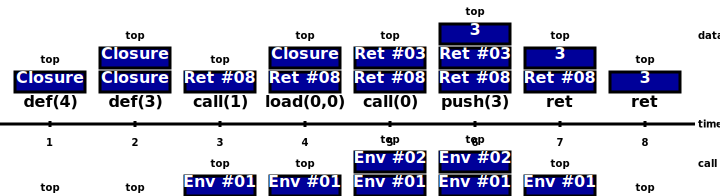
\includegraphics[width=\linewidth]{images/fava.call2.eps}
\caption{function call mechanism for \texttt{((f)=>f())(()=>3)}.\label{fig:call}}
\end{figure}

以上は、引数の値を関数適用の前に求める\textbf{正格評価}の説明である。非正格評価では、引数の値を計算せずに関数を呼ぶ。
条件分岐を含む関数では、引数の値が使用されず廃棄される場合がある。非正格評価であれば、この無駄を解消できる。

\begin{Verbatim}{sample}
fava$ ((x,y,z)=>(x?y:z))(true,3+3,3*3)
6
\end{Verbatim}

引数を無名関数で包み、引数を参照する際にその関数を呼べば、非正格評価と同じ挙動になる。これを\textbf{名前呼び}と呼ぶ。

\begin{Verbatim}{sample}
fava$ ((x,y)=>x()*x()+y())(()=>3+3,()=>3*3)
45
\end{Verbatim}

同じ引数を何度も参照する場合は、値を再利用すると効率的である。これを\textbf{必要呼び}と呼ぶ。詳細は\sectref{lazy}に述べる。

\begin{Verbatim}{sample}
fava$ compile(((x)=>x)(5))
Def(11,1) Load(0,0) Nil Skin(6) Ref Call(0) Load(0,0) Fix Set Get Ret Def(3,0) Push(5) Ret Arg Call(1)
\end{Verbatim}

\chapter{仮想計算機を作る\label{chap:VM}}

\chapref{VM}では、\sectref{pola}で実装した逆ポーランド記法の計算機を拡張し、\chapref{call}の分岐命令を備えた\textbf{仮想計算機}を実装する。
\texttt{FaVM}型が仮想計算機の本体である。\figref{call}と同じ2個のスタックを備え、\textbf{プログラムカウンタ}が示す命令を実行する。

\begin{Verbatim}{Scala}
class FaVM(val codes: Seq[Code], var pc: Int = 0) {
	val call = new Stack[Env]
	val data = new Stack[Any]
	while(pc < codes.size) codes(pc)(this)
}
\end{Verbatim}

\texttt{Stack}型はスタックを実装する。指定された個数の値を取り出す機能や、指定された型で値を取り出す機能を実装する。

\begin{Verbatim}{Scala}
class Stack[E] extends collection.mutable.Stack[E] {
	def popN(n: Int) = Seq.fill(n)(pop).reverse
	def popAs[Type]: Type = pop.asInstanceOf[Type]
	def topAs[Type]: Type = top.asInstanceOf[Type]
	def env = (this :+ null).top.asInstanceOf[Env]
}
\end{Verbatim}

命令は\texttt{Code}型を継承する。仮想計算機の参照を受け取り、所定の操作を実行する。最後に命令を読み取る位置を進める。

\begin{Verbatim}{Scala}
class Code(op: FaVM => Unit) {
	def apply(vm: FaVM) = (op(vm), vm.pc += 1)
}
\end{Verbatim}

\textbf{演算命令}は、値をスタックから取り出して、計算結果をスタックに積む。\textbf{算術演算}と\textbf{論理演算}と\textbf{関係演算}に分類できる。
演算命令は\texttt{ALU}型を継承する。演算命令は\textbf{型検査}も行う。部分関数の使用は型検査が目的で、型次第では例外を起こす。

\begin{Verbatim}{Scala}
class ALU(n: Int, s: String, f: PartialFunction[Seq[Any], Any]) extends Code(vm => {
	def err(v: Seq[_]) = v.map(s => s"$s: ${s.getClass}").mkString("(", ", ", ")")
	vm.data.push(f.applyOrElse(vm.data.popN(n), (v: Seq[_]) => sys.error(err(v))))
})
\end{Verbatim}

分岐命令は\texttt{Jump}型を継承する。引数に渡された関数が整数を返す場合は、命令を読み取る位置を整数の位置に変更する。

\begin{Verbatim}{Scala}
class Jump(op: FaVM => Option[Int]) extends Code(vm => op(vm).foreach(to => vm.pc = to - 1))
\end{Verbatim}

次に、関数の仕組みを実装する。関数は、関数の冒頭の位置と、引数の個数と、関数を生成した時点の環境を参照する。
関数が参照する環境は、この関数を包み込む関数の引数を格納した環境である。関数閉包を実現するための布石である。

\begin{Verbatim}{Scala}
case class Closure(from: Int, narg: Int, out: Env)
\end{Verbatim}

遅延評価の仕組みも実装する。引数の式を包む関数と、計算結果を格納する。これを\textbf{プロミス}と呼ぶ。以下に実装する。

\begin{Verbatim}{Scala}
case class Promise(thunk: Closure, var cache: Any = null, var empty: Boolean = true)
\end{Verbatim}

最後に環境を実装する。環境は、関数適用の際に構築され、関数の引数を記憶する。遅延評価ではプロミスを管理する。
関数閉包の機能を実現するため、環境は連鎖構造を持つ。環境は、関数の包含関係と連動し、\textbf{静的スコープ}を構成する。

\begin{Verbatim}{Scala}
case class Env(args: Seq[Any], out: Env = null) {
	def apply(nest: Int, index: Int): Any = if(nest > 0) out(nest - 1, index) else args(index)
}
\end{Verbatim}

\chapter{命令セットを作る\label{chap:ISA}}

\chapref{ISA}では、\chapref{VM}に述べた仮想計算機に演算命令と分岐命令と遅延評価の命令を実装し、専用の\textbf{命令セット}を構築する。
まず、最も基本的な\texttt{Push}命令を実装する。引数に指定された\textbf{即値}をスタックに積む。定数式は\texttt{Push}命令で実現できる。

\begin{Verbatim}{Scala}
case class Push(v: Any) extends Code(vm => vm.data.push(v))
\end{Verbatim}

機械語では、命令を\textbf{オペコード}と呼び、命令の引数を\textbf{オペランド}と呼ぶ。\sectref{jump}の分岐命令にも、類似した引数がある。

\section{演算命令の設計}

演算命令には単項演算と2項演算がある。単項演算はスタックから値を1個だけ取り出し、計算結果をスタックに戻す。
数値の符号を反転させる\texttt{Neg}命令の実装例を示す。他には\texttt{Pos}命令と論理演算の\texttt{Not}命令もあるが、誌面では省略する。

\begin{Verbatim}{Scala}
case object Neg extends ALU(1, "-", {
	case Seq(v: I) => - v
	case Seq(v: D) => - v
})
\end{Verbatim}

演算命令は型検査も担当する。被演算子が部分関数に列挙するどの型とも異なる場合は、\texttt{ALU}型の内部で例外が起こる。
なお、実装の本筋とは無関係だが、型検査の条件分岐の式を綺麗に揃える目的で、基本型に1文字ずつ別名を設定した。

\begin{Verbatim}{Scala}
import java.lang.{String=>S}, scala.{Any=>A, Int=>I, Double=>D, Boolean=>B}
\end{Verbatim}

2項演算は2個の値を取り出し、計算結果をスタックに戻す。最初に、\texttt{Add}命令を始め5種類の算術演算命令を実装する。
減算や除算を実装する際は、被演算子の順序に注意を要する。演算子の左側の値が\texttt{lhs}に、右側の値が\texttt{rhs}に渡される。

\begin{Verbatim}{Scala}
case object Add extends ALU(2, "+", {
	case Seq(lhs: I, rhs: I) => lhs + rhs
	case Seq(lhs: I, rhs: D) => lhs + rhs
	case Seq(lhs: D, rhs: I) => lhs + rhs
	case Seq(lhs: D, rhs: D) => lhs + rhs
	case Seq(lhs: S, rhs: A) => s"$lhs$rhs"
	case Seq(lhs: A, rhs: S) => s"$lhs$rhs"
})
\end{Verbatim}

次に、関係演算命令を実装する。同値関係を調べる関係演算命令2種類と、順序関係を調べる関係演算命令4種類がある。

\begin{Verbatim}{Scala}
case object Gt extends ALU(2, ">", {
	case Seq(lhs: I, rhs: I) => lhs > rhs
	case Seq(lhs: I, rhs: D) => lhs > rhs
	case Seq(lhs: D, rhs: I) => lhs > rhs
	case Seq(lhs: D, rhs: D) => lhs > rhs
	case Seq(lhs: S, rhs: S) => lhs > rhs
})
\end{Verbatim}

最後に、2種類の論理演算命令を実装する。論理積と論理和である。整数値の場合は2進数の論理積と論理和を計算する。

\begin{Verbatim}{Scala}
case object Or extends ALU(2, "|", {
	case Seq(lhs: B, rhs: B) => lhs | rhs
	case Seq(lhs: I, rhs: I) => lhs | rhs
})
\end{Verbatim}

\section{分岐命令の設計\label{sect:jump}}

分岐命令は\chapref{call}に準拠する。\texttt{Skip}命令は、条件分岐で真の場合の処理を実行した後で、条件分岐を脱出する際に使う。
\texttt{Skin}命令は、値をスタックから取り出し、偽の場合は指定された個数の命令を読み飛ばす。条件分岐や遅延評価で使う。

\begin{Verbatim}{Scala}
case class Skip(plus: Int) extends Jump(vm => Some(vm.pc + plus))
case class Skin(plus: Int) extends Jump(vm => Option.when(!vm.data.popAs[B])(vm.pc + plus))
\end{Verbatim}

\texttt{Def}命令は、指定された個数の引数を取る関数を生成する。関数の開始位置と環境を保存し、関数定義の直後に脱出する。

\begin{Verbatim}{Scala}
case class Def(size: Int, narg: Int) extends Jump(vm => Some {
	vm.data.push(Closure(vm.pc + 1, narg, vm.call.env))
	vm.pc + size
})
\end{Verbatim}

\texttt{Ret}命令は、関数定義の最後に配置される。関数の環境を廃棄して、関数を呼ぶ直前の状態を復元し、以前の位置に戻る。

\begin{Verbatim}{Scala}
case object Ret extends Jump(vm => Some {
	vm.call.remove(0).asInstanceOf[Env]
	vm.data.remove(1).asInstanceOf[Int]
})
\end{Verbatim}

\texttt{Call}命令は、指定された個数の引数で環境を構築する。関数から復帰する際の位置を控え、関数の開始位置に移動する。

\begin{Verbatim}{Scala}
case class Call(argc: Int) extends Jump(vm => Some {
	val args = vm.data.popN(argc)
	val func = vm.data.popAs[Closure]
	vm.call.push(Env(args, func.out))
	vm.data.push(vm.pc + 1)
	if(args.size == func.narg) func.from
	else sys.error(s"${func.narg} arguments required")
})
\end{Verbatim}

正格評価の場合は、\sectref{jump}に実装した分岐命令と、\sectref{lazy}に実装する\texttt{Load}命令があれば、任意の計算を実行できる。

\section{遅延評価の設計\label{sect:lazy}}

最初に、関数の引数を参照する\texttt{Load}命令を実装する。現在の環境の連鎖構造を辿り、指定された番号の引数を取り出す。

\begin{Verbatim}{Scala}
case class Load(nest: Int, id: Int) extends Code(vm => vm.data.push(vm.call.env(nest, id)))
\end{Verbatim}

\texttt{Arg}命令は、関数をスタックから取り出し、値が未定の引数とする。この命令は、関数適用の直前に実行する想定である。

\begin{Verbatim}{Scala}
case object Arg extends Code(vm => vm.data.push(Promise(vm.data.popAs[Closure])))
\end{Verbatim}

\texttt{Get}命令は、引数をスタックから回収して、引数の値をスタックに積む。引数の値は、事前に計算済みである必要がある。
引数の値が計算済みか確認するには、\texttt{Nil}命令を使う。計算が必要な場合は、次に実装する\texttt{Ref}命令を利用して計算する。

\begin{Verbatim}{Scala}
case object Get extends Code(vm => vm.data.push(vm.data.popAs[Promise].cache))
case object Nil extends Code(vm => vm.data.push(vm.data.topAs[Promise].empty))
case object Ref extends Code(vm => vm.data.push(vm.data.topAs[Promise].thunk))
\end{Verbatim}

\texttt{Ref}命令は、引数の実体である関数を取り出す。\texttt{Ref}命令を実行した直後に\texttt{Call}命令を実行すれば、引数の値が求まる。
\texttt{Set}命令は、引数に値を設定する。\texttt{Ref}命令と\texttt{Call}命令で計算した結果を引数に設定すれば、非正格評価を実現できる。

\begin{Verbatim}{Scala}
case object Set extends Code(vm => vm.data.popAs[Promise].cache = vm.data.pop)
case object Fix extends Code(vm => vm.data.topAs[Promise].empty = false)
\end{Verbatim}

\chapter{コンパイラを作る\label{chap:favac}}

\chapref{favac}では、\chapref{fava}の仕様に従って、式を\chapref{ISA}の命令列に翻訳する仕組みを作る。構文解析には\sectref{parsec}の実装を使う。
最初に、\sectref{OpST}から\sectref{CallST}で、様々な構文木を実装する。構文木は、分割統治法によるコード生成器の役割を兼ねる。

\begin{Verbatim}{Scala}
trait AST {
	def code(implicit env: DefST): Seq[Code]
}
\end{Verbatim}

引数\texttt{env}は、その構文木が表す式を包む最も内側の関数を表す。関数の引数を探す場合は、関数を外向きに辿って探す。

\section{定数と演算の構文木\label{sect:OpST}}

算術演算や関係演算や論理演算の式は、逆ポーランド記法の命令列に翻訳される。まず、定数を表す構文木を実装する。

\begin{Verbatim}{Scala}
case class LitST(value: Any) extends AST {
	def code(implicit env: DefST) = Seq(Push(value))
}
\end{Verbatim}

定数は単に\texttt{Push}命令に翻訳される。なお、文字列の場合は、特別に\texttt{StrST}型で扱う。特殊文字の処理を行う目的である。

\begin{Verbatim}{Scala}
case class StrST(string: String) extends AST {
	def code(implicit env: DefST) = LitST(StringContext.processEscapes(string)).code
}
\end{Verbatim}

次に、演算子の構文木を実装する。単項演算は\texttt{UnST}型で表す。被演算子の命令列を生成し、直後に演算命令を追加する。

\begin{Verbatim}{Scala}
case class UnST(op: String, expr: AST) extends AST {
	def code(implicit env: DefST) = op match {
		case "+" => expr.code :+ Pos
		case "-" => expr.code :+ Neg
		case "!" => expr.code :+ Not
	}
}
\end{Verbatim}

2項演算は\texttt{BinST}型で表す。まず左側の被演算子の、次に右側の被演算子の命令列を生成し、直後に演算命令を追加する。

\begin{Verbatim}{Scala}
case class BinST(op: String, e1: AST, e2: AST) extends AST {
	def code(implicit env: DefST) = op match {
		case "+"  => e1.code ++ e2.code :+ Add
		case "-"  => e1.code ++ e2.code :+ Sub
		case "*"  => e1.code ++ e2.code :+ Mul
		case "/"  => e1.code ++ e2.code :+ Div
		case "%"  => e1.code ++ e2.code :+ Mod
		case "&"  => e1.code ++ e2.code :+ And
		case "|"  => e1.code ++ e2.code :+ Or
		case ">=" => e1.code ++ e2.code :+ Ge
		case "<=" => e1.code ++ e2.code :+ Le
		case ">"  => e1.code ++ e2.code :+ Gt
		case "<"  => e1.code ++ e2.code :+ Lt
		case "==" => e1.code ++ e2.code :+ Eq
		case "!=" => e1.code ++ e2.code :+ Ne
	}
}
\end{Verbatim}

条件分岐の式は\texttt{IfST}型で表す。条件式と、真の場合に評価する式と、偽の場合に評価する式で、合計3個の引数を取る。

\begin{Verbatim}{Scala}
case class IfST(cond: AST, v1: AST, v2: AST) extends AST {
	def code(implicit env: DefST) = {
		val (code1, code2) = v1.code -> v2.code
		val jmp1 = Skin(2 + code1.size) +: code1
		val jmp2 = Skip(1 + code2.size) +: code2
		cond.code ++ jmp1 ++ jmp2
	}
}
\end{Verbatim}

条件分岐は、条件式の命令列の後に、\texttt{Skin}命令と、真の場合の命令列と、\texttt{Skip}命令と、偽の場合の命令列を出力する。

\section{関数と引数の構文木\label{sect:CallST}}

最初に、関数を表す\texttt{DefST}型を実装する。引数と、関数の内容を引数に取る。また、外側の関数を参照する変数を持つ。
関数の内容の命令列を生成してから、その長さと引数の個数に対応した\texttt{Def}命令と、\texttt{Ret}命令を冒頭と最後に追加する。

\begin{Verbatim}{Scala}
case class DefST(pars: Seq[String], body: AST, var out: DefST = null) extends AST {
	def code(implicit env: DefST) = {
		val codes = body.code((this.out = env, this)._2)
		(Def(codes.size + 2, pars.size) +: codes :+ Ret)
	}
}
\end{Verbatim}

関数は、定義された際の関数の包含関係を保持する。最も外側の関数は、便宜的に架空の関数を表す\texttt{Root}型を参照する。

\begin{Verbatim}{Scala}
object Root extends DefST(Seq(), null)
\end{Verbatim}

次に、識別子の構文木を実装する。正格評価の場合は\texttt{StIdST}型を使う。関数の包含構造を外向きに遡り、仮引数を探す。

\begin{Verbatim}{Scala}
case class StIdST(val name: String) extends AST {
	def search(env: DefST, nest: Int = 0): Load = {
		val idx = env.pars.indexOf(name)
		if(idx >= 0) return Load(nest, idx)
		if(env.out != null) search(env.out, nest + 1)
		else sys.error(s"variable $name not defined")
	}
	def code(implicit env: DefST) = Seq(search(env))
}
\end{Verbatim}

非正格評価の場合は\texttt{LzIdSt}型を使う。引数を取り出し、計算が必要なら計算し、引数の値を取り出す命令列を生成する。

\begin{Verbatim}{Scala}
case class LzIdST(val name: StIdST) extends AST {
	val (head, tail) = Seq(Nil, Skin(6), Ref, Call(0)) -> Seq(Fix, Set, Get)
	def code(implicit env: DefST) = (name.code ++ head ++ name.code ++ tail)
}
\end{Verbatim}

非正格評価の場合は、関数に渡す実引数を関数に包む必要がある。関数の命令列を生成し、直後に\texttt{Arg}命令を配置する。

\begin{Verbatim}{Scala}
case class LzArgST(body: AST) extends AST {
	def code(implicit env: DefST) = DefST(Seq(), body).code :+ Arg
}
\end{Verbatim}

\texttt{CallST}型は、関数適用を表す。まず、関数を参照する式の、次に引数の命令列を展開し、最後に\texttt{Call}命令を配置する。

\begin{Verbatim}{Scala}
case class CallST(f: AST, args: Seq[AST]) extends AST {
	def code(implicit env: DefST) = f.code ++ args.map(_.code).flatten :+ Call(args.size)
}
\end{Verbatim}

\section{再帰下降構文解析器}

最後に、\sectref{parsec}で実装した解析表現文法の構文解析器を組み合わせ、再帰下降構文解析器を構築する。以下に実装する。
\chapref{fava}に掲載した文法の定義とほぼ同じ構造である。ただし、左結合の演算子は\texttt{Fold}型を利用して、左再帰を回避した。

\begin{Verbatim}{Scala}
object FavaPEGs extends PEGs {
	def expr: PEG[AST] = (cond / or) <~ ("//" ~ ".*$".r).?
	def cond = (or <~ "?") ~ expr ~ (":" ~> expr) ^ (c->y->n => IfST(c, y, n))
	def or   = new Fold(and, "|" ^ (op => BinST(op, _, _)))
	def and  = new Fold(eql, "&" ^ (op => BinST(op, _, _)))
	def eql  = new Fold(rel, """(!|=)=""".r ^ (op => BinST(op, _, _)))
	def rel  = new Fold(add, """[<>]=?""".r ^ (op => BinST(op, _, _)))
	def add  = new Fold(mul, """[\+\-]""".r ^ (op => BinST(op, _, _)))
	def mul  = new Fold(unr, """[\*/%]""".r ^ (op => BinST(op, _, _)))
	def unr  = ("+" / "-" / "!").* ~ call ^ (o->e => o.foldRight(e)(UnST))
	def call = fact ~ args.* ^ (f->a => a.foldLeft(f)(CallST))
	def args = "(" ~> new Sep(expr ^ LzArgST, ",") <~")"
	def fact = func / bool / text / real / int / name / ("(" ~> expr <~ ")")
	def func = pars ~ ("=>" ~> expr) ^ (p->e => DefST(p, e))
	def pars = "(" ~> new Sep(name, ",") <~ ")" ^ (_.map(_.name.name))
	def bool = ("true" / "false") ^ (_.toBoolean) ^ LitST
	def text = ("\"" ~> """([^"\\]|\\[\\'"bfnrt])*""".r <~ "\"") ^ StrST
	def int  = """\d+""".r ^ (_.toInt) ^ LitST
	def real = """(\d+\.\d*|\d*\.\d+)""".r ^ (_.toDouble) ^ LitST
	def name = """[@A-Z_a-z][@0-9A-Z_a-z]*""".r ^ StIdST ^ LzIdST
}
\end{Verbatim}

使用例を以下に示す。構文解析を実行し、命令列に翻訳して\chapref{VM}で実装した仮想計算機に渡すと、計算が実行される。

\begin{Verbatim}{Scala}
println(new FaVM(FavaPEGs.expr("((x,y)=>x+y)(2,3)").get.m.code(Root)).data.pop)
\end{Verbatim}

この構文解析器に、特殊な命令として\texttt{compile}を追加して、命令列を文字列で出力する機能を実装すれば、完成である。

\section{言語処理系を動かす}

完成した言語処理系は、\chapref{lambda}に述べたラムダ計算の実験環境として利用できる。まず、\eqref{num}の自然数の演算を試す。
自然数は帰納的に枚挙可能で、自然数の後続の自然数を求める関数と$0$で表現できる。加算と乗算も、簡単に実装できる。

\begin{Verbatim}{sample}
fava$ ((l,r)=>(f,x)=>l(f)(r(f)(x)))((f)=>(x)=>f(x),(f)=>(x)=>f(f(x)))((x)=>x+1,0) // 1 + 2
3
fava$ ((l,r)=>(f,x)=>l(r(f))(x))((f)=>(x)=>f(f(x)),(f)=>(x)=>f(f(x)))((x)=>x+1,0) // 2 * 2
4
\end{Verbatim}

次に、\eqref{bool}の真偽値の演算を試す。真偽値は、真と偽の順序組で表現できる。論理積と論理和も、簡単に実装できる。

\begin{Verbatim}{sample}
fava$ ((l,r)=>l(r,(x,y)=>y))((x,y)=>x,(x,y)=>y)(true,false) // true & false
false
fava$ ((l,r)=>l((x,y)=>x,r))((x,y)=>x,(x,y)=>y)(true,false) // true | false
true
\end{Verbatim}

無名関数による再帰計算も可能である。\eqref{Y}に述べた不動点演算子を利用する。$10$の階乗を求める例を以下に示す。

\begin{Verbatim}{sample}
fava$ ((f)=>((x)=>f(x(x)))((x)=>f(x(x))))((f)=>(n)=>(n==0)?1:n*f(n-1))(10)
3628800
\end{Verbatim}

正格評価の言語では、無限再帰に陥る。代替手段として\eqref{Z}の不動点演算子を利用すれば、再帰計算が可能になる。

\begin{Verbatim}{sample}
fava$ ((f)=>((x)=>f((y)=>x(x)(y)))((x)=>f((y)=>x(x)(y))))((f)=>(n)=>(n==0)?1:n*f(n-1))(10)
3628800
\end{Verbatim}

\end{document}
